\begin{figure}[!htb]
\begin{center}
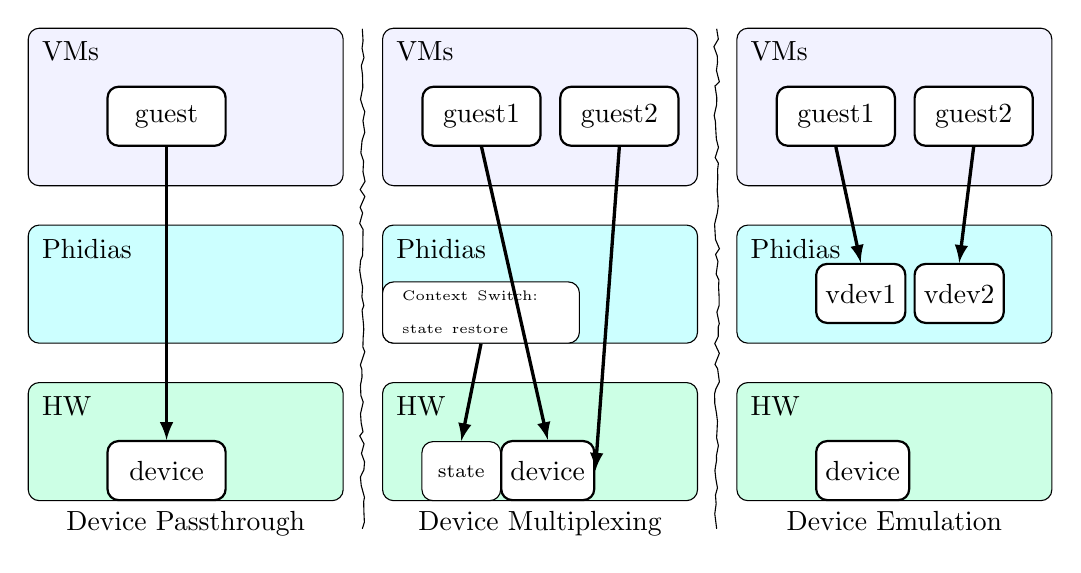
\begin{tikzpicture}

\node at (0,4)[rectangle, draw=black, fill=Blue!5, rounded corners, minimum height = 2cm, minimum width = 4cm, anchor=south west] (vms1) {};
\node[below right, inner sep=5pt] at (vms1.north west) {VMs};
\node at (4.5,4)[rectangle, draw=black, fill=Blue!5, rounded corners, minimum height = 2cm, minimum width = 4cm, anchor=south west] (vms2) {};
\node[below right, inner sep=5pt] at (vms2.north west) {VMs};
\node at (9,4)[rectangle, draw=black, fill=Blue!5, rounded corners, minimum height = 2cm, minimum width = 4cm, anchor=south west] (vms3) {};
\node[below right, inner sep=5pt] at (vms3.north west) {VMs};

\node at (0,2)[rectangle, draw=black, fill=Cyan!20, rounded corners, minimum height = 1.5cm, minimum width = 4cm, anchor=south west] (phidias1) {};
\node[below right, inner sep=5pt] at (phidias1.north west) {Phidias};
\node at (4.5,2)[rectangle, draw=black, fill=Cyan!20,  rounded corners, minimum height = 1.5cm, minimum width = 4cm, anchor=south west] (phidias2) {};
\node[below right, inner sep=5pt] at (phidias2.north west) {Phidias};
\node at (9,2)[rectangle, draw=black, fill=Cyan!20, rounded corners, minimum height = 1.5cm, minimum width = 4cm, anchor=south west] (phidias3) {};
\node[below right, inner sep=5pt] at (phidias3.north west) {Phidias};

\node at (0,0)[rectangle, draw=black, fill=SpringGreen!20, rounded corners, minimum height = 1.5cm, minimum width = 4cm, label=south:Device Passthrough,anchor=south west] (hw1) {};
\node[below right, inner sep=5pt] at (hw1.north west) {HW};
\node at (4.5,0)[rectangle, draw=black, fill=SpringGreen!20, rounded corners, minimum height = 1.5cm, minimum width = 4cm, label=south:Device Multiplexing, anchor=south west] (hw2) {};
\node[below right, inner sep=5pt] at (hw2.north west) {HW};
\node at (9,0)[rectangle, draw=black, fill=SpringGreen!20, rounded corners, minimum height = 1.5cm, minimum width = 4cm, label=south:Device Emulation, anchor=south west] (hw3) {};
\node[below right, inner sep=5pt] at (hw3.north west) {HW};

\node at (1,4.5)[thick, rectangle, draw=black, fill=white, rounded corners, minimum height = 0.75cm, minimum width = 1.5cm, anchor=south west] (g11) {guest};
\node at (1,0)[thick, rectangle, draw=black, fill=white, rounded corners, minimum height = 0.75cm, minimum width = 1.5cm, anchor=south west] (dev1) {device};
\begin{scope}[>=latex]
	\draw [very thick, ->] (g11.south) to [bend right=0] (dev1.north);
\end{scope}

\node at (5,4.5)[thick, rectangle, draw=black, fill=white, rounded corners, minimum height = 0.75cm, minimum width = 1.5cm, anchor=south west] (g21) {guest1};
\node at (6.75,4.5)[thick, rectangle, draw=black, fill=white, rounded corners, minimum height = 0.75cm, minimum width = 1.5cm, anchor=south west] (g22) {guest2};
\node at (4.5,2.0)[rectangle, draw=black, fill=white,  rounded corners, minimum height = 0.75cm, minimum width = 2.5cm, text width=2cm, anchor=south west] (hyp2st) 
					{\tiny{Context Switch: state restore}};
\node at (5,0)[rectangle, draw=black, fill=white, rounded corners, minimum height = 0.75cm, minimum width = 1cm, anchor=south west] (dev2st) {\scriptsize{state}};
\node at (6,0)[thick, rectangle, draw=black, fill=white, rounded corners, minimum height = 0.75cm, minimum width = 1cm, anchor=south west] (dev2) {device};
\begin{scope}[>=latex]
	\draw [very thick, ->] (g21.south) to [bend right=0] (dev2.north);
	\draw [very thick, ->] (g22.south) to [bend right=0] (dev2.east);
	\draw [very thick, ->] (hyp2st.south) to [bend right=0] (dev2st.north);
\end{scope}


\node at (9.5,4.5)[thick, rectangle, draw=black, fill=white, rounded corners, minimum height = 0.75cm, minimum width = 1.5cm, anchor=south west] (g31) {guest1};
\node at (11.25,4.5)[thick, rectangle, draw=black, fill=white, rounded corners, minimum height = 0.75cm, minimum width = 1.5cm, anchor=south west] (g32) {guest2};
\node at (10,2.25)[thick, rectangle, draw=black, fill=white, rounded corners, minimum height = 0.75cm, minimum width = 1cm, anchor=south west] (vdev1) {vdev1};
\node at (11.25,2.25)[thick, rectangle, draw=black, fill=white, rounded corners, minimum height = 0.75cm, minimum width = 1cm, anchor=south west] (vdev2) {vdev2};
\node at (10,0)[thick, rectangle, draw=black, fill=white, rounded corners, minimum height = 0.75cm, minimum width = 1cm, anchor=south west] (dev3) {device};
\begin{scope}[>=latex]
	\draw [very thick, ->] (g31.south) to [bend right=0] (vdev1.north);
	\draw [very thick, ->] (g32.south) to [bend right=0] (vdev2.north);	
\end{scope}

\draw [decorate, decoration={random steps, segment length=3pt,amplitude=1pt}] (4.25,-0.35) -- (4.25,6);
\draw [decorate, decoration={random steps, segment length=3pt,amplitude=1pt}] (8.75,-0.35) -- (8.75,6);

\end{tikzpicture}
\end{center}
\ifreport
\caption{Device handling mechanisms supported by Phidias}
\fi
\label{fig-device-handling}
\end{figure}
